\documentclass{beamer}

\newtheorem{conjecture}{Conjecture}
 \newcommand{\bconj}[1]{\begin{conj}#1\end{conj}}
\newtheorem{mconj}{Metaconjecture}

\newtheorem{prop}{Proposition}
 \newcommand{\bprop}[1]{\begin{prop}#1\end{prop}}
\newtheorem{lem}{Lemma}
 \newcommand{\blem}[1]{\begin{lem}#1\end{lem}}


\newtheorem{guess}{Guess}
 \newcommand{\bguess}[1]{\begin{guess}#1\end{guess}}
%\newtheorem{corollary}{Corollary}



\usepackage{tikz,framed, amsrefs, amsthm, color,wrapfig}
\tikzstyle{every node}=[circle, draw, fill=black!50,
                        inner sep=0pt, minimum width=4pt]
\tikzstyle{dot}=[circle, draw, fill=black,
                        inner sep=0pt, minimum width=2pt]

\tikzstyle{lblvertex}=[fill=white, inner sep = 1pt, font=\small]
\tikzstyle{lblvertex2}=[fill=white, inner sep = 1pt, font=\tiny,circle, draw]
\tikzstyle{lblvertex3}=[fill=white, inner sep = 1pt, font=\tiny,circle, draw = black!25]
\tikzstyle{words} =[rectangle, draw=none, fill=none, black]
\newcommand{\bframe}[2]{\begin{frame}{#1}#2\end{frame}}
\newcommand{\bfig}[2]{\begin{figure}#1\caption{#2}\end{figure}}


\usetheme{CambridgeUS}
\setbeamertemplate{navigation symbols}{}
\usecolortheme[RGB={216,30,5}]{structure}
\AtBeginSection[] % "Beamer, do the following at the start of every section"
{
\begin{frame}<beamer>
\frametitle{Outline} % make a frame titled "Outline"
\tableofcontents[currentsection] % show TOC and highlight current section
\end{frame}
}

\title{Connected matchings in special families of graphs}
\author{Chris Caragianis}
\institute[U of L]{ Department of Mathematics\\ University of Louisville\\ Louisville, KY 40292\\[1ex]
   \texttt{cjcara01@louisville.edu} }
\begin{document}
\bframe{Ordered connected matchings}{

\begin{center}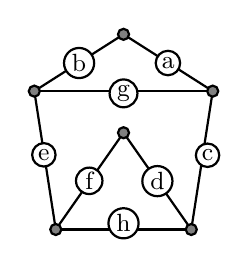
\begin{tikzpicture}[thick,scale=0.5]

	\coordinate (a) at (90:2.5);
	\coordinate (b) at (25:2.5); 
	\coordinate (c) at (0:0);
	\coordinate (d) at (155:2.5);
	\coordinate (e) at (-55:3);
	\coordinate (f) at (-125:3);

	\coordinate (A) at (57.5:2.1);

	\draw (a)--(b);\draw (57.5:2.1)node [lblvertex]{a};
	%\draw (b)--(c);
	\draw (d)--(a); \draw (122.5:2.1)node [lblvertex]{b};
	%\draw (a)--(c);
	%\draw (c)--(d);
	\draw (b)--(e); \draw (-15:2.21)node [lblvertex]{c};
	\draw (e)--(c); \draw (-55:1.5)node [lblvertex]{d};
	\draw (d)--(f);\draw (195.5:2.1)node [lblvertex]{e};
	\draw (f)--(c); \draw (-125.5:1.5)node [lblvertex]{f};
	\draw (d)--(b); \draw (90:1)node [lblvertex]{g};
	\draw (e)--(f); \draw (-90:2.3)node [lblvertex]{h};
	%\draw (f) arc {-125:-33:3};
	
	\draw (a) node {};
	\draw (b) node {};
	\draw (c) node {};
	\draw (d) node {};
	\draw (e) node {};
	\draw (f) node {};
	
\end{tikzpicture}
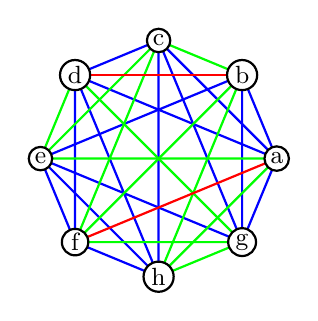
\begin{tikzpicture}[thick,scale=0.5]

	\coordinate (a) at (0:3);
	\coordinate (b) at (45:3); 
	\coordinate (c) at (90:3);
	\coordinate (d) at (135:3);
	\coordinate (e) at (180:3);
	\coordinate (f) at (225:3);
	\coordinate (h) at (270:3);
	\coordinate (g) at (315:3);

	\draw[blue] (a) -- (b) -- (e) -- (f) -- (d) -- (c) -- (a) -- (d);
	\draw[blue] (a) -- (g) -- (b) ;
	\draw[blue] (a) -- (c) -- (g) -- (e) -- (h) -- (d);
	\draw[blue] (c) -- (h) --(f);
	\draw[green] (a) -- (e) --(c) -- (f) -- (g) -- (h) -- (b) -- (h) -- (a);
	\draw[green] (g)--(d) -- (e);
	\draw[green] (c) -- (b) -- (f);
	\draw[red] (b)--(d);
	\draw[red](a)--(f);
	\draw (a) node[lblvertex] {a};
	\draw (b) node[lblvertex] {b};
	\draw (c) node[lblvertex] {c};
	\draw (d) node[lblvertex] {d};
	\draw (e) node[lblvertex] {e};
	\draw (f) node[lblvertex] {f};
	\draw (g) node[lblvertex] {g};
	\draw (h) node[lblvertex] {h};
\end{tikzpicture}
\end{center}\pause\vskip 0.5 cm

}

\end{document}